%%%%%%%%%%%%%%%%%%%%%%%%%%%%%
\section{能量差 $\Delta{}E$和束流约束质量$M_{\rm BC}$}

我们用前面列出的判选条件挑出所有满足条件的\basic,然后根据~$\lambdacp$ 重子的衰变模式来组合这些次级粒子,得到各个衰变道的~$\lambdacp$ 的候选者。
我们在$D$-tagging软件包的基础上进行了改造,开发出了~$\lambdacp$-tagging 软件包。
$\lambdacp$--tagging 软件包是~BESIII 上粲重子物理研究的重要工具,大部分的~$\lambdacp$ 相关物理分析都采用了基于它重建的~$\lambdacp$ 重子。
这一分析工具可以将所有$\lambdacp$衰变道的所有候选~$\lambdacp$的信息都保存下来。
我们可以对这些候选~$\lambdacp$ 做进一步的筛选,进行相关的物理分析。


通常怎样鉴别一个$\lambdacp$,或说选取一个什么样的变量来区分本底事例和信号事例?
一个自然的想法是查看重建出的$\lambdacp$的不变质量是否在$\lambdacp$的质量处。
在我们的情况中,我们关心的过程末态只有一对$\lambdacp\lambdacm$重子,两个$\lambdacp\lambdacm$重子平分对撞的能量,所以一个$\lambdacp$重子的能量应该等于束流能量。这也是阈值上数据所特有的优势。
束流能量是可以较精确地知道的,其比重建出的$\lambdacp$的能量分辨要好很多。
所以在计算$\lambdacp$的不变质量时可以将重建出的$\lambdacp$的能量用束流能量来代替,这样可以改善分辨。
我们称使用束流能量计算的不变质量为束流约束质量,记为$M_{\rm BC}$。
束流能量还可以提供另外一个关键变量$\Delta E$,它定义为束流能量和重建出的$\lambdacp$的能量差。
它可以用来很好地区分本底和信号:正确重建的$\lambdacp$,其$\Delta E$应当在零附近,其~$M_{\rm BC}$应该在~$\lambdacp$的不变质量中心值附近。
$M_{\rm BC}$和$\Delta E$可以用公式表达为~\cite{CLEO_phase1,CLEO_phase2}:
\begin{equation}
M_{\rm BC} \equiv \sqrt{E_{\rm beam}^{2}/c^{4}-p_{\lambdacp}^{2}/c^{2}},
\end{equation}
\begin{equation}
\Delta E\equiv E_{\lambdacp}-E_{\rm beam},
\end{equation}
其中 $p_{\lambdacp}$ 和 $E_{\lambdacp}$ 是重建出的$\lambdacp$的所有末态粒子动量和能量之和(在~$e^{+}e^{-}$ 质心系中), $E_{\rm beam}$ 表示束流能量。
我们通过拟合$M_{\rm BC}$的分布来获得数据中的$\lambdacp$产额。
经过初步挑选,我们以$\Lmodeb$为例画出数据中和纯信号过程中$\Delta E$的分布如图~\ref{fig:deltaE}所示。
如前所述,正确重建的$\lambdacp$信号,$\Delta E$应该在0附近。
我们通过比较数据中和纯信号过程中$\Delta E$分布,考虑信号区约为$\pm$3$\sigma$以内,进而确定了$\Delta E$信号区,列在表~\ref{tab:STyields}中。

%%%%%%%%%%%%%%%%%%%%%%%%%%%%
\begin{figure*}[hp]
\centering
\subfigure[]
{
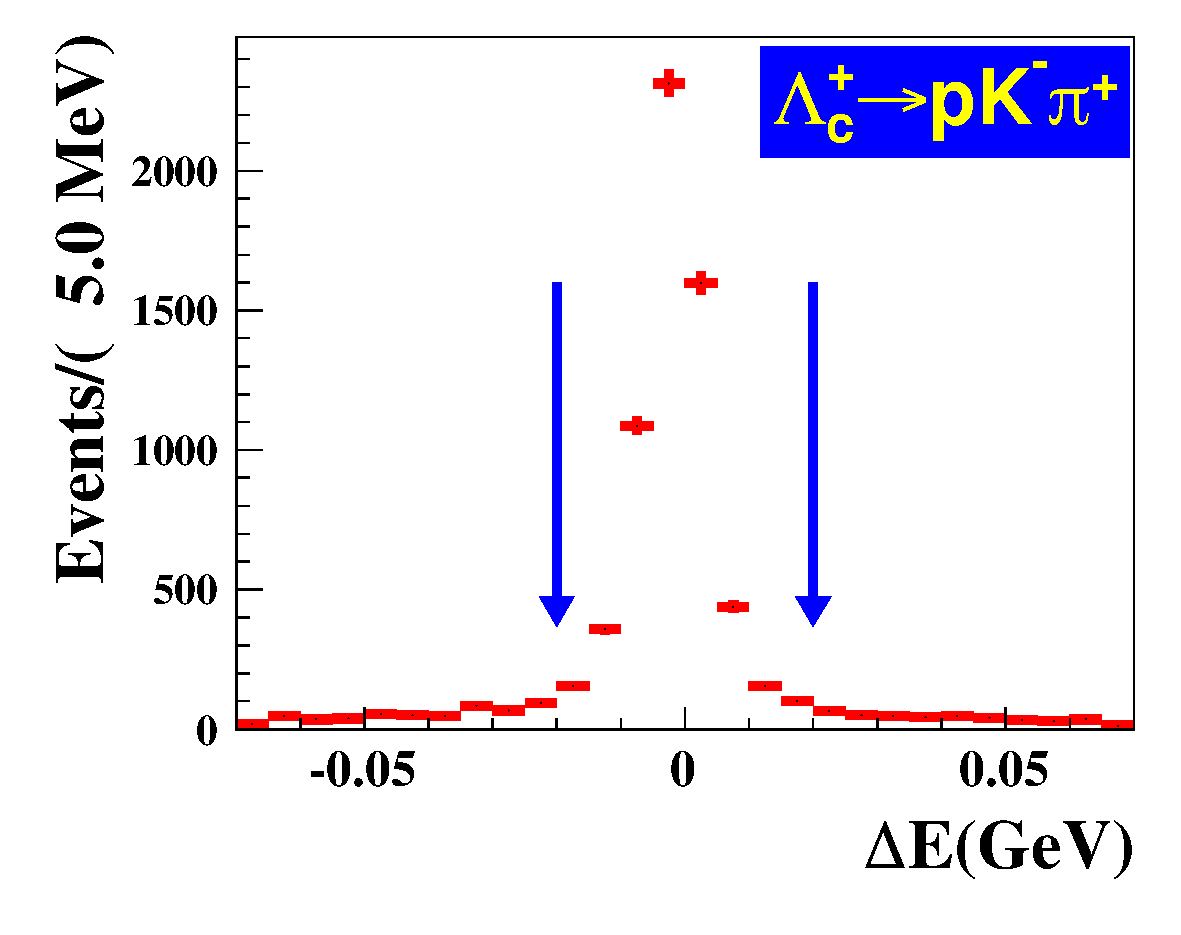
\includegraphics[width=0.4\textwidth]{chap2_data_deltaE_mode1}
}
\subfigure[]
{
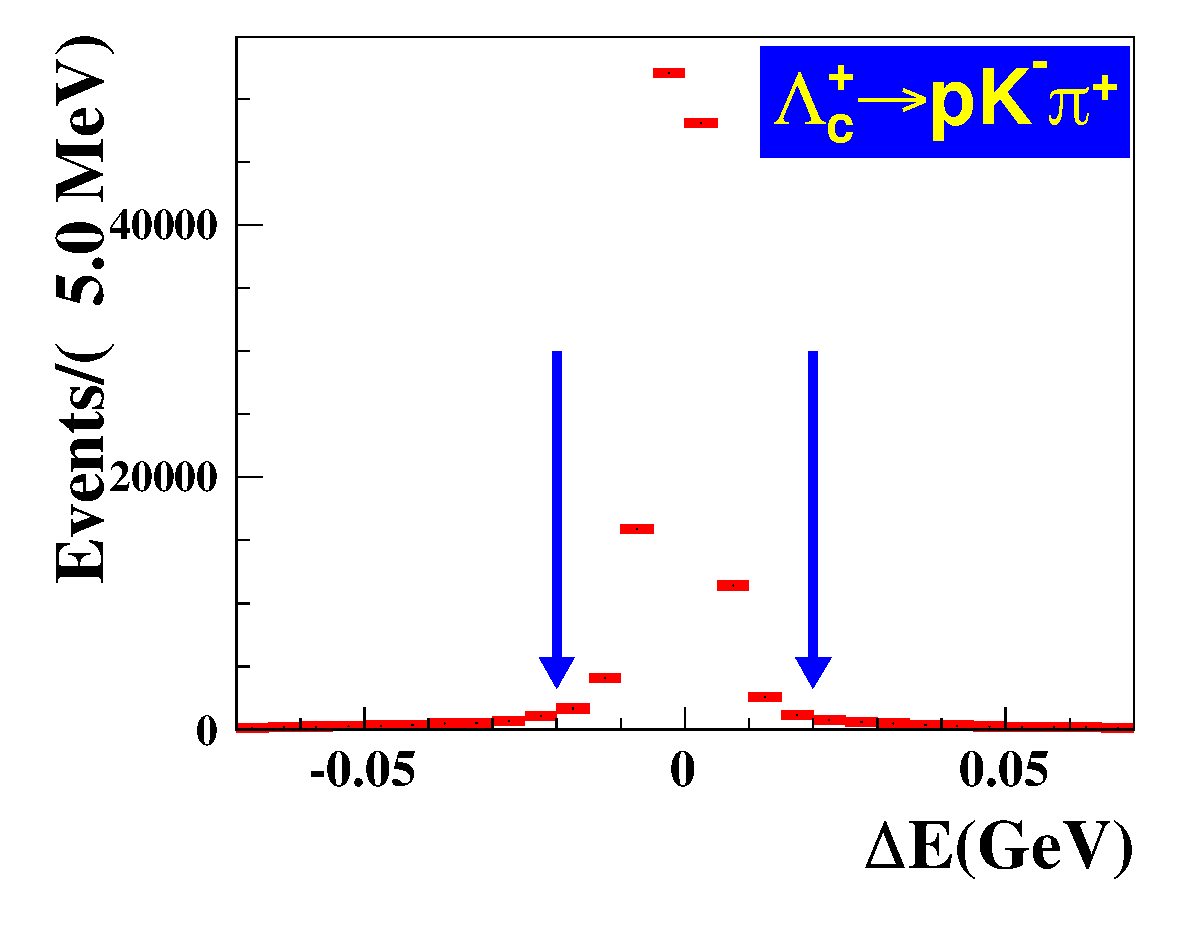
\includegraphics[width=0.4\textwidth]{chap2_sigmc_deltaE_mode1}
}
\caption{$\Lmodeb$衰变中$\Delta{}E$的分布,左图为数据中的分布,右图为单标记信号MC的分布。图中箭头指示了信号区间。}
\label{fig:deltaE}
\end{figure*}


%%%%%%%%%%%%%%%%%%%%%%%%%%%%%%%%%%%%%%%
\begin{table}[H]
  \begin{center}
  %\footnotesize
 \caption{单标记$\lambdacp$的$\Delta{}E$要求, 单标记产额$N_{i}^{\rm ST}$以及单标记$\varepsilon_{i}^{\rm ST}$。 双标记效率$\varepsilon_{i,\Xi K}^{\rm DT}$ 和双标记效率$\varepsilon_{i,\Xi^{*}K}^{\rm DT}$。误差只包含统计误差。效率不包含任何中间共振态的分支比$\mathcal{B}$。}
  \resizebox{\linewidth}{!}{
  \begin{tabular}{l|c|c|c|c|c}
      \hline \hline
  衰变道  &$\Delta{}E$ (MeV) & $N_{i}^{\rm ST}$ & $\varepsilon_{i}^{\rm ST}(\%)$ & $\varepsilon_{i,\Xi K}^{\rm DT}(\%)$  & $\varepsilon_{i,\Xi^{*}K}^{\rm DT}(\%)$\\ \hline
$\textbf{$\modea$}$ & $(-20,20)$ & $1145\pm34$ & $51.6$ & $41.2$ & $42.6$  \\
$\textbf{$\modeb$}$ & $(-20,20)$ & $5722\pm80$ & $45.2$ & $37.3$ & $39.1$ \\
$\textbf{$\modec$}$ & $(-30,20)$ & $478\pm28$ & $17.2$ & $15.1$ & $15.2$ \\
$\textbf{$\moded$}$ & $(-20,20)$ & $431\pm25$ & $18.6$ & $15.4$ & $15.2$ \\
$\textbf{$\modee$}$ & $(-30,20)$ & $1407\pm51$ & $14.7$ & $13.4$ & $12.7$ \\
$\textbf{$\modef$}$ & $(-20,20)$ & $474\pm41$ & $55.4$ & $43.3$ & $45.1$ \\
$\textbf{$\modeaa$}$ & $(-20,20)$ & $648\pm25$ & $38.7$ & $30.9$ & $31.4$ \\
$\textbf{$\modebb$}$ & $(-30,20)$ & $1282\pm43$ & $13.0$ & $10.9$ & $11.2$ \\
$\textbf{$\modedd$}$ & $(-20,20)$ & $540\pm27$ & $10.6$ & $9.0$ & $8.8$ \\
$\textbf{$\modeaaa$}$ & $(-20,20)$ & $427\pm23$ & $24.1$ & $20.6$ & $20.6$ \\
$\textbf{$\modeccc$}$ & $(-50,30)$ & $258\pm20$ & $19.6$ & $17.3$ & $17.4$ \\
$\textbf{$\modeddd$}$ & $(-30,20)$ & $1005\pm42$ & $20.1$ & $17.2$ & $18.1$ \\ 
\hline  \hline
   \end{tabular}
   }
   \label{tab:STyields}
  \end{center}
  \end{table}

